\documentclass[conference]{IEEEtran}
\IEEEoverridecommandlockouts
% The preceding line is only needed to identify funding in the first footnote. If that is unneeded, please comment it out.
\usepackage{cite}
\usepackage{amsmath,amssymb,amsfonts}
\usepackage{algorithmic}
\usepackage{graphicx}
\usepackage{textcomp}
\usepackage{xcolor}
\usepackage[brazilian]{babel}
\usepackage[utf8]{inputenc}
\usepackage[T1]{fontenc}
\usepackage{listings}
\usepackage{color}
\usepackage{float}
\usepackage{multirow}
\usepackage{hyperref}

\definecolor{dkgreen}{rgb}{0,0.6,0}
\definecolor{gray}{rgb}{0.5,0.5,0.5}
\definecolor{mauve}{rgb}{0.58,0,0.82}

\lstset{frame=tb,
  language=Java,
  aboveskip=3mm,
  belowskip=3mm,
  showstringspaces=false,
  columns=flexible,
  basicstyle={\small\ttfamily},
  numbers=none,
  numberstyle=\tiny\color{gray},
  keywordstyle=\color{blue},
  commentstyle=\color{dkgreen},
  stringstyle=\color{mauve},
  breaklines=true,
  breakatwhitespace=true,
  tabsize=3
}
\lstset{language=Python}
\def\BibTeX{{\rm B\kern-.05em{\sc i\kern-.025em b}\kern-.08em
    T\kern-.1667em\lower.7ex\hbox{E}\kern-.125emX}}
\begin{document}

\title{Relatório do Laboratório 13: \\ Deep Q-Learning\\
}

\author{\IEEEauthorblockN{Isabelle Ferreira de Oliveira}
\IEEEauthorblockA{\textit{CT-213 - Engenharia da Computação 2020} \\
\textit{Instituto Tecnológico de Aeronáutica (ITA)}\\
São José dos Campos, Brasil \\
isabelle.ferreira3000@gmail.com}
}

\maketitle

\begin{abstract}
Esse relatório documenta a resolução do problema de Mountain Car no ambiente OpenAI Gym usando o algoritmo seminal de Deep Reinforcement Learning: o Deep Q-Learning/Deep Q-Networks (DQN).
\end{abstract}

\begin{IEEEkeywords}
Mountain Car, OpenAI Gym, Deep Reinforcement Learning, Deep Q-Learning, Deep Q-Networks
\end{IEEEkeywords}

\section{Implementação}

	\subsection{Implementação da Definição da Rede Neural}
	
	Essa primeira etapa se tratou da implementação do método build\underline{\space}model() da classe DQNAgent de dqn\underline{\space}agent.py, script fornecido no código base do laboratório. Nesse método, era preciso construir uma rede em Keras de acordo com as especificações apresentadas na Tabela 3 do roteiro do laboratório \cite{roteiro}.
	
	Essa implementação foi feita de forma bastante análoga à maneira do laboratório 8 \cite{roteiro8}, ou seja, seguindo o apresentado no pseudo-código em Python a seguir.
	
\begin{lstlisting}
# Adds the first layer
model.add(layers.Dense(num_neurons,
	activation=activations.some_function,
	input_dim=state_size))

# Adds another layer (not first)
model.add(layers.Dense(num_neurons,
	activation=activations.some_function))
\end{lstlisting}

	Vale ressaltar que, para atender os critérios requisitados, some\underline{\space}function do pseudo-código acima se tratou de \textit{relu} para as duas primeiras camadas, e de \textit{linear} para terceira camada. Além disso, num\underline{\space}neurons foram 24, 24 e action\underline{\space}size para as primeira, segunda e terceira camada, respectivamente.

	Fora isso, bastou-se descomentar as linhas de criação de uma pilha linear de camadas, as linhas compilação do modelo e impressão do summary do modelo, apresentado futuramente na seção Resultados e Conclusões \ref{results}, e a linha de retorno da função.

	\subsection{Escolha de Ação usando Rede Neural}

Para realizar o aprendizado do robô seguidor de linha, utilizando as duas técnicas implementadas anteriormente (Sarsa e Q-Learning), foi executado o script main.py, alterando-se o valor da variável rl\underline{\space}algorithm, entre os construtores: Sarsa e QLearning, com seus respectivos parâmetros.

		\subsection{Reward Engineering}

		\subsection{Treinamento usando DQN}

		\subsection{Avaliação da Política}

\section{Resultados e Conclusões} \label{results}

	\subsection{Implementação dos algoritmos de RL}

Conforme apresentado nas Figuras \ref{sarsa_test_rl} e \ref{qlearning_test_rl}, pode-se observar resultados equivalentes para ambas as técnicas. Assim, tanto a tabela de action-value possuiu valores similares, como as sequências de ações foram idênticas nas duas situações. Nota-se também que quanto mais perto do objetivo, maior o valor da action-value.

\begin{figure}[htbp]
\centering
\centerline{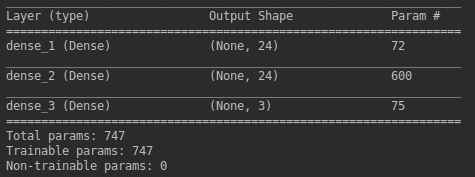
\includegraphics[scale=0.5]{imagens/summary.png}}
\caption{Sumário do modelo implementado em Keras.}.
\label{summary}
\end{figure}

\begin{figure}[htbp]
\centering
\centerline{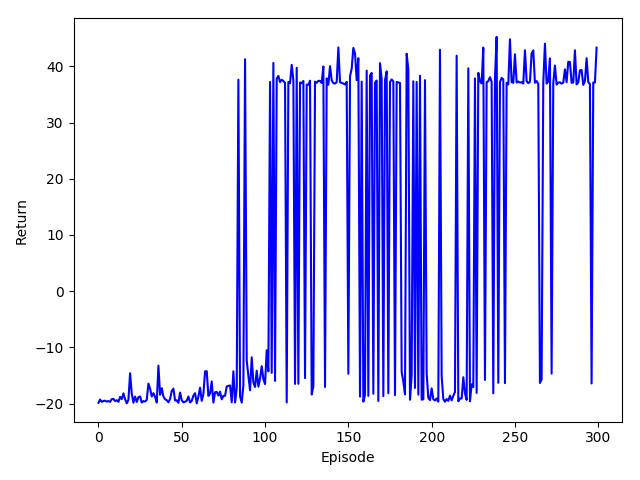
\includegraphics[scale=0.3]{imagens/train/15.png}}
\caption{Gráfico gerado a partir do treinamento do modelo para 300 episódios.}.
\label{train/15}
\end{figure} 

	\subsection{Escolha de Ação usando Rede Neural}

Os resultados do aprendizado da política do robô seguidor de linha, utilizando os algoritmos de Sarsa e Q-Learning estão representados nas Figuras de \ref{sarsa/action_value_table} a \ref{sarsa/line_follower_solution} e \ref{q-learning/action_value_table} a \ref{q-learning/line_follower_solution}, respectivamente.

Comparando as tabelas de action-value para os dois algoritmos, em \ref{sarsa/action_value_table} e \ref{q-learning/action_value_table}, pode-se notar a quase equivalência entre os resultados. Nota-se também que quanto mais perto do objetivo, maior o valor da action-value. Nas Figuras \ref{sarsa/greedy_policy_table} e \ref{q-learning/greedy_policy_table}, a tendência das duas também são semelhantes, embora já se consiga ver mais claramente algumas diferenças, nada que prejudique o processo de aprendizado.

Por fim, as Figuras \ref{sarsa/return_convergence} e \ref{q-learning/return_convergence} comprovam a convergência (até consideravelmente rápida) dos métodos, chegando aos resultados de caminho apresentados nas Figuras \ref{sarsa/line_follower_solution} e \ref{q-learning/line_follower_solution} para Sarsa e Q-Learning, respectivamente.

Esses resultados foram obtidos após 500 iterações no algoritmo Sarsa, e 556 no algoritmo Q-Learning, e demonstraram a correta implementação do código e funcionalidade para problemas de aprendizado por reforço.

\begin{figure}[htbp]
\centering
\centerline{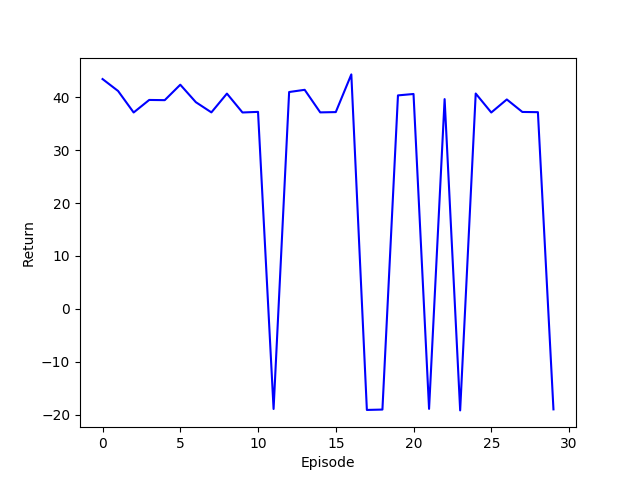
\includegraphics[scale=0.5]{imagens/dqn_evaluation.png}}
\caption{Representação em cores da tabela de action-value calculada, para algoritmo de Sarsa.}.
\label{dqn_evaluation}
\end{figure}

\begin{figure}[htbp]
\centering
\centerline{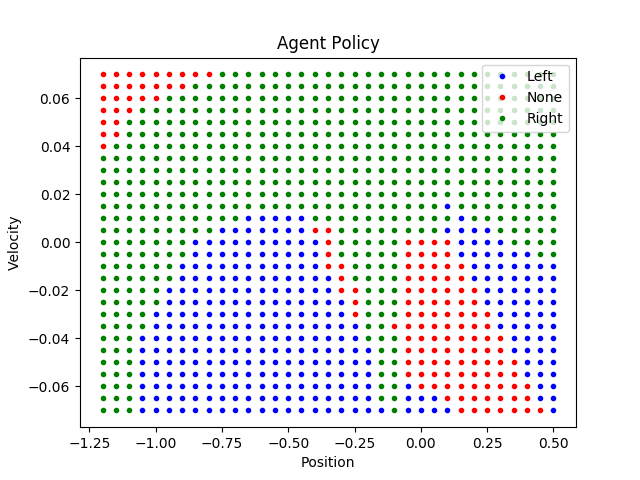
\includegraphics[scale=0.5]{imagens/agent_decision.png}}
\caption{Representação em cores da tabela de greedy-policy calculada, para algoritmo de Sarsa.}.
\label{agent_decision}
\end{figure} 

\begin{figure}[htbp]
\centering
\centerline{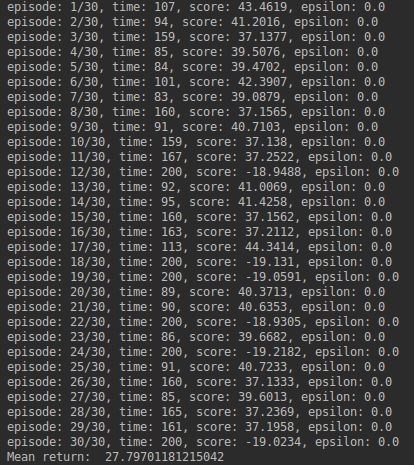
\includegraphics[scale=0.4]{imagens/evaluate_dqn_result.png}}
\caption{Recompensa acumulada em função das iterações, para algoritmo de Sarsa.}.
\label{evaluate_dqn_result}
\end{figure}

	\subsection{Reward Engineering}

	\subsection{Treinamento usando DQN}
	
	\subsection{Avaliação da Política}
	
\begin{thebibliography}{00}
\bibitem{roteiro} M. Maximo, ``Roteiro: Laboratório 12 - Deep Q-Learning''. Instituto Tecnológico de Aeronáutica, Departamento de Computação. CT-213, 2019.

\bibitem{roteiro8} M. Maximo, ``Roteiro: Laboratório 8 - Imitation Learning com Keras''. Instituto Tecnológico de Aeronáutica, Departamento de Computação. CT-213, 2019.

\end{thebibliography}

\end{document}
